\documentclass{book}

% Configuration
% ------------------
% Packages
% ------------------
\usepackage[english]{babel}
\usepackage[T1]{fontenc}
\usepackage[scaled]{helvet}
\usepackage[utf8]{inputenc}
\usepackage[letterpaper]{geometry}
\usepackage[dvipsnames]{xcolor}

\usepackage{algorithmicx}
\usepackage{algpseudocode}
\usepackage{amsfonts,amsmath,amsthm,amssymb}
\usepackage{booktabs}
\usepackage{float}
\usepackage{graphicx}
\usepackage{latexsym}
\usepackage{mathtools}
\usepackage{sectsty}
\usepackage{setspace}
\usepackage{subcaption}
\usepackage{tabularx}
\usepackage{tikz}
% \usepackage{txfonts}
\usepackage{url}
\usepackage{wrapfig}
\usepackage{xparse}

% ------------------
% Shortcuts
% ------------------

% ------------------
% Command Redefinitions
% ------------------
\renewcommand{\qed}{\hfill$\blacksquare$}

\makeatletter
\renewcommand*\env@matrix[1][*\c@MaxMatrixCols c]{%
    \hskip -\arraycolsep
    \let\@ifnextchar\new@ifnextchar
    \array{#1}}
\makeatother

% ------------------
% Colors
% ------------------
\definecolor{primary}{HTML}{207BA5}
\definecolor{greybg}{RGB}{249, 249, 249}

\definecolor{thmbg}{HTML}{F2F2F9}
\definecolor{lemmabg}{HTML}{FFFAF8}
\definecolor{lemmafr}{HTML}{983b0f}
\definecolor{propbg}{HTML}{f2fbfc}
\definecolor{propfr}{HTML}{191971}
\definecolor{myp}{RGB}{197, 92, 212}
\definecolor{grey17}{RGB}{17, 17, 17}
\definecolor{MyGrey}{HTML}{5B5B5B}

\definecolor{lightBlue}{rgb}{0.0, 0.64, 1.0}
\definecolor{lightRed}{rgb}{1.0, 0.50, 0.50}
\definecolor{darkGreen}{rgb}{0.31, 0.54, 0.30}
\definecolor{violet}{RGB}{186, 153, 242}

%----------------
%	Text Styles
%----------------
\DeclareTextFontCommand{\term}{\color{orange}\bfseries}
\DeclareTextFontCommand{\bred}{\color{red}\bfseries}
\DeclareTextFontCommand{\itblue}{\color{lightBlue}\itshape}

\DeclareTextFontCommand{\vector}{\bfseries\itshape}

% ------------------
%   URL Color
% ------------------
\usepackage[colorlinks=true]{hyperref}
\hypersetup{
    colorlinks=true,
    linkcolor=black,
    filecolor=magenta,
    urlcolor=blue,
}

% ------------------
% Tikz Externalize
% ------------------
\usetikzlibrary{external}
\tikzexternalize[prefix=tikz/]
\tikzset{external/only named=true}

% ------------------
% Boxes
% ------------------
\usepackage[most]{tcolorbox}

\newcommand\fancybox[3]{%
    \tcbset{
        mybox/.style={
                enhanced,
                boxsep=0mm,
                opacityfill=0,
                overlay={
                        \coordinate (X) at ([xshift=-1mm, yshift=-1.5mm]frame.north west);
                        \node[align=right, text=#1, text width=2.5cm, anchor=north east] at (X) {\bf#2};
                        \draw[line width=0.5mm, color=#1] (frame.north west) -- (frame.south west);
                    }
            }
    }
    \begin{tcolorbox}[mybox]
        #3
    \end{tcolorbox}
}

\tcbuselibrary{theorems,skins,hooks}
\NewDocumentCommand\thmbox{m O{\Large #1} O{greybg} O{primary} O{number within=section}}
{
    \newtcbtheorem[#5]{#1}{\large #2}
    {%
        enhanced,
        breakable,
        colback = #3,
        frame hidden,
        boxrule = 0sp,
        borderline west = {2pt}{0pt}{#4},
        sharp corners,
        detach title,
        before upper = \tcbtitle\par\smallskip,
        coltitle = #4,
        fonttitle = \bfseries,
        %description font = \mdseries,
        separator sign none,
        segmentation style={solid, #4}
    }
    {th}
}

\thmbox{Corollary}[Corollary][myp!10][myp!85!black]
\thmbox{Lemma}[Lemma][lemmabg][lemmafr]
\thmbox{Propo}[Proposition][propbg][propfr]
\thmbox{Defi}[Definition][primary!12][primary]
\thmbox{Notation}[Notation][white][grey17][no counter]
\thmbox{Theorem}[Theorem][primary!12][primary]
\thmbox{Remark}[Remark][grey17!10][grey17][no counter]

% ------------------
% Environments
% ------------------
\newenvironment{corollary}[1][]   {\begin{Corollary}{#1}{}}                               {\end{Corollary}}
\newenvironment{definition}[1][]  {\begin{Defi}{#1}{}}                                    {\end{Defi}}
\newenvironment{lemma}[1][]       {\begin{Lemma}{#1}{}}                                   {\end{Lemma}}
\newenvironment{proposition}[1][] {\begin{Propo}{#1}{}}                                   {\end{Propo}}
\newenvironment{remark}[1][]      {\begin{Remark}{#1}{}}                                  {\end{Remark}}
\newenvironment{theorem}[1][]     {\begin{Theorem}{#1}{}}                                 {\end{Theorem}}

\newenvironment{rtheorem}[2][]    {\begin{Theorem}{#1}{#2}}                               {\end{Theorem}}

\theoremstyle{definition}
\newtheorem*{exam}{\color{primary}Example}
% \newcommand{\example}[1]{\begin{exam}#1\end{exam}}
% \newenvironment{example}          {\begin{exam}} {\begin{flushright}${\color{primary}\diamondsuit}$\end{flushright} \end{exam}}
\newenvironment{example}          {\begin{exam}} {\hfill${\color{primary}\diamondsuit}$\end{exam}}

\theoremstyle{definition}
\newtheorem*{clm}{\color{MyGrey}Claim}
\newenvironment{claim}            {\begin{clm}} {\end{clm}}

% ------------------
% Lists
% ------------------
\usepackage{enumitem}

\newcommand{\cnumero}[2]{
    \tikz[baseline=(myanchor.base)]
    \node[minimum size=0.2cm,circle,
        inner sep=1pt,draw, #2,thick,fill=#2](myanchor)
    {\color{white}\bfseries\fontsize{8}{8}#1};}

\newcommand*{\itembolasazules}[1]{\protect\cnumero{#1}{primary}}

\newenvironment{listo} {\begin{enumerate}[label=\itembolasazules{\arabic*}]} {\end{enumerate}}
\newenvironment{listu} {\begin{itemize}  [label=$\color{primary} \bullet$]}  {\end{itemize}}

% ------------------
% Table of Contents
% ------------------
\usepackage{blindtext}
\usepackage{framed}
\usepackage{titletoc}
\usepackage{etoolbox}

\patchcmd{\tableofcontents}{\contentsname}{\contentsname}{}{}

\renewenvironment{leftbar}
{\def\FrameCommand{\hspace{6em}%
        {\color{primary}\vrule width 2pt depth 6pt}\hspace{1em}}%
    \MakeFramed{\parshape 1 0cm \dimexpr\textwidth-6em\relax\FrameRestore}\vskip2pt%
}
{\endMakeFramed}

\titlecontents{chapter}[0em]
{\vspace*{2\baselineskip}}
{\parbox{4.5em}{%
        \hfill\Huge\bfseries\color{primary}\thecontentslabel}%
    \vspace*{-2.3\baselineskip}\leftbar\textbf{\color{primary}\small\chaptername~\thecontentslabel}\\
}{}{\endleftbar}

\titlecontents{section}[8.4em]
{\contentslabel{3em}}{}{}
{\hspace{0.5em}\nobreak\itshape\color{primary}\contentspage}

\titlecontents{subsection}[11.4em]
{\contentslabel{3em}}{}{}
{\hspace{0.5em}\nobreak\itshape\color{primary}\contentspage}

% ------------------
% Chapters
% ------------------
\newtcolorbox{titlecolorbox}[1]{ %the box around chapter
    coltext=white,
    colframe=primary,
    colback=primary,
    boxrule=0pt,
    arc=0pt,
    notitle,
    width=4.8em,
    height=2.4ex,
    before=\hfill
}

\usepackage[explicit]{titlesec}

\makeatletter
\let\old@rule\@rule
\def\@rule[#1]#2#3{\textcolor{primary}{\old@rule[#1]{#2}{#3}}}
\makeatother

\titleformat{\chapter}[display]
{\Huge}
{}
{0pt}
{\begin{titlecolorbox}{}
        {\large\MakeUppercase{\bf\chaptername}}
    \end{titlecolorbox}
    \vspace*{-3.19ex}\noindent\rule{\textwidth}{0.4pt}
    \parbox[b]{\dimexpr\textwidth-4.8em\relax}{\raggedright\MakeUppercase{#1}}{\hfill\fontsize{70}{60}\selectfont{\color{primary}\thechapter}}
}
[]

\titleformat{name=\chapter,numberless}[display]
{\Huge}
{}
{0pt}
{
    \vspace*{-3.19ex}\noindent\rule{\textwidth}{0.4pt}
    \parbox[b]{\dimexpr\textwidth-4.8em\relax}{\raggedright\MakeUppercase{#1}}
}
[]

% ------------------
% Sections
% ------------------
\titleformat{\section}[hang]{\Large\bfseries}%
{\rlap{\color{primary}\rule[-6pt]{\textwidth}{0.4pt}}\colorbox{primary}{%
        \raisebox{0pt}[13pt][3pt]{ \makebox[60pt]{% height, width
                \selectfont\color{white}{\thesection}}
        }}}%
{15pt}%
{ \color{primary}#1
    %
}
\titlespacing*{\section}{0pt}{3mm}{5mm}
% ------------------
% Subsections
% ------------------
\subsectionfont{\Large\color{primary}}

% ------------------
% Bibliography and Index
% ------------------
\usepackage{csquotes}
\usepackage[
    style=alphabetic, 
    citestyle=numeric,
    sorting=nyt,
    sortcites=true,
    autopunct=true,
    autolang=hyphen,
    hyperref=true,
    abbreviate=false,
    backref=true,
    backend=biber,
    defernumbers=true
]{biblatex}
\addbibresource{./bibliography.bib} % BibTeX bibliography file
\defbibheading{bibempty}{}

\usepackage{calc} % For simpler calculation - used for spacing the index letter headings correctly
\usepackage{makeidx} % Required to make an index
\makeindex % Tells LaTeX to create the files required for indexing

% ------------------
% Title page
% ------------------
\usetikzlibrary{calc}
\usetikzlibrary{shapes.geometric}
\usepackage{anyfontsize}
\newcommand{\frontpage}[3]{
    \begin{tikzpicture}[remember picture, overlay]
        % Background
        \fill[primary] (current page.south west) rectangle (current page.north east);

        \foreach \i in {2.5,...,22} {
            \node[rounded corners,primary!60,draw,regular polygon,regular polygon sides=6, minimum size=\i cm,ultra thick] at ($(current page.west)+(2.5,-5)$) {} ;
        }

        % Background Polygon
        \foreach \i in {0.5,...,22} {
            \node[rounded corners,primary!60,draw,regular polygon,regular polygon sides=6, minimum size=\i cm,ultra thick] at ($(current page.north west)+(2.5,0)$) {} ;
        }

        \foreach \i in {0.5,...,22} {
            \node[rounded corners,primary!90,draw,regular polygon,regular polygon sides=6, minimum size=\i cm,ultra thick] at ($(current page.north east)+(0,-9.5)$) {} ;
        }

        \foreach \i in {21,...,6} {
            \node[primary!85,rounded corners,draw,regular polygon,regular polygon sides=6, minimum size=\i cm,ultra thick] at ($(current page.south east)+(-0.2,-0.45)$) {} ;
        }

        % Title
        \node[left,primary!5,minimum width=0.625*\paperwidth,minimum height=3cm, rounded corners] at ($(current page.north east)+(0,-9.5)$) {
            {\fontsize{25}{30} \selectfont \bfseries #1}
        };

        % Subtitle
        \node[left,primary!10,minimum width=0.625*\paperwidth,minimum height=2cm, rounded corners] at ($(current page.north east)+(0,-11)$) {
            {\huge \textit{#2}}
        };

        % Author
        \node[left,primary!5,minimum width=0.625*\paperwidth,minimum height=2cm, rounded corners] at ($(current page.north east)+(0,-13)$) {
            {\Large \textsc{#3}}
        };

        % Year
        \node[rounded corners,fill=primary!70,text =primary!5,regular polygon,regular polygon sides=6, minimum size=2.5 cm,inner sep=0,ultra thick] at ($(current page.west)+(2.5,-5)$) {\LARGE \bfseries \the\year{}};
    \end{tikzpicture}
}


\begin{document}

\pagestyle{empty}
\frontpage{CSC320}{Introduction to Visual Computing}{Sinan Li}
\newpage

\tableofcontents
\newpage

\tikzset{
    graph-node/.style={
        circle,
        fill=red,
        draw=black,
        line width=0.5pt,
        inner sep=1.5pt
    },
    every edge/.style={
        draw,
        thick,
    },
    non-edge/.style={
        dotted,
        lightBlue,
    },
}

\part{Foundations}

\chapter{Image Geometry}

\section{Linear 2D Transforms}

\subsection{Homogeneous 2D Point Coordinate}

\subsubsection{Basic Notational Conventions}

\begin{listu}
    \item Column-Vector Representation \[
        \begin{bmatrix}
            x \\
            y 
        \end{bmatrix}
    \]

    \item Row-Vector Representation \[
        \begin{bmatrix}
            x & y
        \end{bmatrix}
    \]

    \item Matrix Transpose Operation \[
        \begin{bmatrix}
            x \\
            y
        \end{bmatrix}^\top = \begin{bmatrix}
            x & y
        \end{bmatrix}
    \]
\end{listu}

\subsubsection{Homogeneous Coordinates}

In the standard Euclidean coordinate system, a point is represented by a pair of coordinates $(x, y)$, where $x$ and $y$ are the coordinates of the point along the $x$ and $y$ axes, respectively. 

\begin{center}
    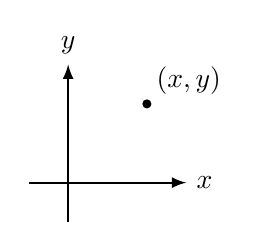
\begin{tikzpicture}[scale=0.5]
        \draw[thick,>=latex,->] (-1, 0) -- (3, 0) node[right] {$x$};
        \draw[thick,>=latex,->] (0, -1) -- (0, 3) node[above] {$y$};
        \draw[fill=black] (2, 2) circle (0.1) node[above right] {$(x, y)$};
    \end{tikzpicture}
\end{center}

In homogeneous coordinates, a point is represented by a triple of coordinates $(x, y, w)$, where $x$ and $y$ are the coordinates of the point along the $x$ and $y$ axes, respectively, and $w$ is a scaling factor that is normally set to $1$. The homogeneous coordinates of a point are not unique, since any multiple of the coordinates $(x, y, w)$ represents the same point. For example, $(2, 3, 1)$ and $(4, 6, 2)$ represent the same point. The homogeneous coordinates of a point are unique only up to a scaling factor. 

\begin{remark}
    Two vector of homogeneous coordinates $(x, y, w)$ and $(x', y', w')$ represent the same point if and only if there exists a non-zero scalar $\lambda$ such that \[
        \begin{bmatrix}
            x \\
            y \\
            w
        \end{bmatrix} = \lambda \begin{bmatrix}
            x' \\
            y' \\
            w'
        \end{bmatrix}
    \]
\end{remark}

\begin{example}
    The homogeneous coordinates of the point $(2, 3)$ are $(2, 3, 1)$, $(4, 6, 2)$, $(6, 9, 3)$, etc.
\end{example}

\subsubsection{Homogeneous to Euclidean Coordinat}

To convert a homogeneous coordinate $(x, y, w)$ to a Euclidean coordinate $(x', y')$, we divide the first two coordinates of the homogeneous coordinate by the third coordinate, i.e. \[
    \begin{bmatrix}
        x' \\
        y'
    \end{bmatrix} = \begin{bmatrix}
        x / w \\
        y / w
    \end{bmatrix}
\]

\begin{example}
    Plot the following points in the Euclidean plane: \[
        \begin{matrix}[l l l]
            P_1 = (2, 2, 2) & P_2 = (10, 0, 2) & P_3 = (0, 8, 4) \\
            P_4 = (1, 0, 0.01) & P_5 = (1, 0, 0) & P_6 = (0, 1, 0) \\
            P_7 = (1, 1, 0) & &
        \end{matrix}
    \]

    \begin{center}
        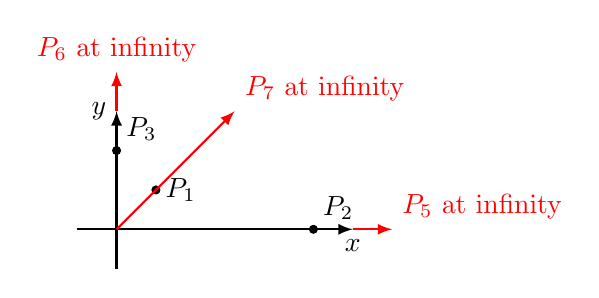
\begin{tikzpicture}[scale=0.5]
            \draw[thick,>=latex,->] (-1, 0) -- (6, 0) node[below] {$x$};
            \draw[thick,>=latex,->] (0, -1) -- (0, 3) node[left] {$y$};

            \draw[fill=black] (1, 1) circle (0.1) node[right] {$P_1$};
            \draw[fill=black] (5, 0) circle (0.1) node[above right] {$P_2$};
            \draw[fill=black] (0, 2) circle (0.1) node[above right] {$P_3$};

            \draw[thick,>=latex,->,red] (6, 0) -- (7, 0) node[above right] {$P_5$ at infinity};
            \draw[thick,>=latex,->,red] (0, 3) -- (0, 4) node[above] {$P_6$ at infinity};
            % P7
            \draw[thick,>=latex,->,red] (0, 0) -- (3, 3) node[above right] {$P_7$ at infinity};
        \end{tikzpicture}
    \end{center}

    Note that $P_5$, $P_6$, and $P_7$ are at infinity. This is a very important property of homogeneous coordinates. 
\end{example}

\begin{remark}
    Points infinitely far away from the origin in the Euclidean plane have a finite representation in homogeneous coordinates (i.e. $(x, y, 0)$). These points are sometimes called \term{ideal points}.
\end{remark}

\subsection{Homogeneous 2D Line Coordinates}

\subsubsection{Homogeneous 2D Line Coordinates}

\begin{remark}
    The general equation of a line in the Euclidean plane is \[
        ax + by + c = 0
    \] where $a$, $b$, and $c$ are real numbers and $a$ and $b$ are not both zero.

    In homogeneous coordinates, using the matrix notation, the general equation of a line is \[
        \begin{bmatrix}
            a & b & c
        \end{bmatrix} \begin{bmatrix}
            x \\ y \\ w
        \end{bmatrix} = 0
    \]
    Or, equivalently, \[
        \ell^\top p = 0
    \] where $\ell$ is the vector holding line coefficients and $p$ is the vector holding point coordinates.
\end{remark}

\begin{definition}
    The \term{homogeneous coordinates of a line} with the equation \[ ax + by + c = 0 \] is the vector \[ \ell = \begin{bmatrix} a \\ b \\ c \end{bmatrix} \]
\end{definition}

\begin{example}
    The homogeneous coordinates of the line $y = x$ is \[
        \ell = \begin{bmatrix}
            -1 \\ 1 \\ 0
        \end{bmatrix}
    \]
\end{example}

\subsubsection{Line Passing Through Two Points}

In this case, $\ell$ must satisfy the following equations: \[
    \ell^\top P_1 = 0 \qquad \ell^\top P_2 = 0
\] where $p_1$ and $p_2$ are the homogeneous coordinates of the two points.

We can take the cross product of $p_1$ and $p_2$ to obtain $\ell$: \[
    \ell = P_1 \times P_2
\]

\begin{remark}
    To compute the cross product of two vectors, we can use the following two methods. 

    \[
        \ell = \begin{bmatrix}
            x_1 \\ y_1 \\ z_1
        \end{bmatrix} \times \begin{bmatrix}
            x_2 \\ y_2 \\ z_2
        \end{bmatrix}
    \]

    {~~~}

    \begin{minipage}[t]{0.45\linewidth}
        As matrix multiplication: \[
            P_1 \times P_2 = \begin{bmatrix}
                0 & -z_1 & y_1 \\
                z_1 & 0 & -x_1 \\
                -y_1 & x_1 & 0
            \end{bmatrix} P_2
        \]
    \end{minipage}%
    \hfil%
    \begin{minipage}[t]{0.45\linewidth}
        As determinant: \[
            P_1 \times P_2 = \left| 
                \begin{matrix}
                    \color{red} i & \color{red} j & \color{red} k \\
                    x_1 & y_1 & z_1 \\
                    x_2 & y_2 & z_2
                \end{matrix}
            \right|
        \]
    \end{minipage}
\end{remark}

\subsubsection{Intersection of Two Lines}

In this case, $p$ must satisfy the following equations: \[
    \ell_1^\top p = 0 \qquad \ell_2^\top p = 0
\] where $\ell_1$ and $\ell_2$ are the homogeneous coordinates of the two lines.

We can take the cross product of $\ell_1$ and $\ell_2$ to obtain $p$: \[
    p = \ell_1 \times \ell_2
\]

\begin{remark}
    For parallel lines, we cannot compute its standard Euclidean intersection point. Instead, we can compute the homogeneous intersection point, which will be at infinity.
\end{remark}

\subsection{Affine 2D Transformations}

\begin{listu}
    \item \textbf{Identity} \[
        \begin{bmatrix}
            x' \\ y' \\ w'
        \end{bmatrix} \cong \begin{bmatrix}
            x \\ y \\ 1
        \end{bmatrix} = \begin{bmatrix}
            1 & 0 & 0 \\
            0 & 1 & 0 \\
            0 & 0 & 1
        \end{bmatrix} \begin{bmatrix}
            x \\ y \\ 1
        \end{bmatrix}
    \]

    \item \textbf{Stretching} (along $x$) \[
        \begin{bmatrix}
            x' \\ y' \\ w'
        \end{bmatrix} \cong \begin{bmatrix}
            {\color{red} s} x \\ y \\ 1
        \end{bmatrix} = \begin{bmatrix}
            1 & 0 & {\color{red} t} \\
            0 & 1 & 0 \\
            0 & 0 & 1
        \end{bmatrix} \begin{bmatrix}
            x \\ y \\ 1
        \end{bmatrix}
    \]
    
    \textbf{Stretching} (along $y$) \[
        \begin{bmatrix}
            x' \\ y' \\ w'
        \end{bmatrix} \cong \begin{bmatrix}
            x \\ {\color{red} s} y \\ 1
        \end{bmatrix} = \begin{bmatrix}
            1 & 0 & 0 \\
            0 & {\color{red} s} & 0 \\
            0 & 0 & 1
        \end{bmatrix} \begin{bmatrix}
            x \\ y \\ 1
        \end{bmatrix}
    \]

    \item \textbf{Shearing} (along $y$) \[
        \begin{bmatrix}
            x' \\ y' \\ w'
        \end{bmatrix} \cong \begin{bmatrix}
            x \\ {\color{red} h} x + y \\ 1
        \end{bmatrix} = \begin{bmatrix}
            1 & 0 & 0 \\
            {\color{red} h} & 1 & 0 \\
            0 & 0 & 1
        \end{bmatrix} \begin{bmatrix}
            x \\ y \\ 1
        \end{bmatrix}
    \]

    \item \textbf{Rotation} (about the origin bt angle $\phi$) \[
        \begin{bmatrix}
            x' \\ y' \\ w'
        \end{bmatrix} \cong \begin{bmatrix}
            {\color{red}(\cos \phi)} x {\color{red}- (\sin \phi)} y \\
            {\color{red}(\sin \phi)} x + {\color{red}(\cos \phi)} y \\
            1
        \end{bmatrix} = \begin{bmatrix}
            {\color{red}\cos \theta} & {\color{red}-\sin \theta} & 0 \\
            {\color{red}\sin \theta} & {\color{red}\cos \theta} & 0 \\
            0 & 0 & 1
        \end{bmatrix} \begin{bmatrix}
            x \\ y \\ 1
        \end{bmatrix}
    \]

    \item \textbf{Translation} (along $x$) \[
        \begin{bmatrix}
            x' \\ y' \\ w'
        \end{bmatrix} \cong \begin{bmatrix}
            x + {\color{red} d} \\ y \\ 1
        \end{bmatrix} = \begin{bmatrix}
            1 & 0 & {\color{red} d} \\
            0 & 1 & 0 \\
            0 & 0 & 1
        \end{bmatrix} \begin{bmatrix}
            x \\ y \\ 1
        \end{bmatrix}
    \]

    \textbf{Translation} (along $y$) \[
        \begin{bmatrix}
            x' \\ y' \\ w'
        \end{bmatrix} \cong \begin{bmatrix}
            x \\ y + {\color{red} d} \\ 1
        \end{bmatrix} = \begin{bmatrix}
            1 & 0 & 0 \\
            0 & 1 & {\color{red} d} \\
            0 & 0 & 1
        \end{bmatrix} \begin{bmatrix}
            x \\ y \\ 1
        \end{bmatrix}
    \]
\end{listu}

We can combine these transformations to form more complex transformations. For example, we can combine a rotation and a translation to form a \term{rotation about a point} transformation. 

\begin{definition}[Affine Transformation (Intuitive)]
    An \term{affine transformation} is any combination of scaling, shearing, rotation, and translation.

    \[ 
        \begin{bmatrix}
            a & b & c \\
            d & e & f \\
            0 & 0 & g
        \end{bmatrix} 
    \] where $g \neq 0$ is a scaling factor that does not affect the transformation.
\end{definition}

\begin{remark}
    An affine transformation is a transformation that preserves parallelism and ratios of distances along parallel lines.
\end{remark}

In the original image, two parallel lines would intersect at some infinity $(x, y, 0)$. After an affine transformation, the two lines would still intersect at some infinity $(x', y', 0)$. \[
    \begin{bmatrix}
        x' \\ y' \\ 0
    \end{bmatrix} = \begin{bmatrix}
        a & b & c \\
        d & e & f \\
        0 & 0 & g
    \end{bmatrix} \begin{bmatrix}
        x \\ y \\ 0
    \end{bmatrix}
\]

\begin{definition}[Affine Transformation]
    An affine transformation is any invertible $3 \times 3$ matrix that preserves the points at infinity.
\end{definition}

But what if the last row of the matrix is not $(0, 0, 1)$?

\subsection{Homographies}

\term{Homographies} are also called \term{projective transformations} or \term{perspective transformations}. They still preserve linearity, but they do not preserve parallelism.

\begin{definition}
    A \term{homography} is any 2D transformation of homogeneous coordinates that is represented by an invertible $3 \times 3$ matrix.

    \[
        \begin{bmatrix}
            a & b & c \\
            d & e & f \\
            l & m & g
        \end{bmatrix}
    \]
\end{definition}

All homographies are invertible. This is because Homographies map unique points to unique points. 

% TODO: Why do lines remain straight after a homography

\begin{remark}
    Lines remain straight after a homography.

    Let $\ell^T p = 0$ be a line. It suffices to show that all points on this line are mapped to points on a line.

    % TODO
\end{remark}

\begin{example}
    A naive image warping algorithm is forward mapping. 

    \begin{verbatim}
input: src_image, H
output: dest_image

for c=1 to num_columns               // cycle over all source pixels
   for r=1 to num_rows
        x, y = pixel_xy(r,c)         // get the source pixel's (x,y) coordinates
        p = homogeneous_coords(x, y) // convert to vector homogeneous coords
        p_prime = H*p                // apply homography
        x_prime, y_prime = euclidean_coords(p_prime)  // convert to Euclidean coords
        r_prime, c_prime = pixel_rc(x_prime, y_prime) // calculate the dest pixel    
        dest_image(r_prime, c_prime) = src_image(r,c) // copy pixel color            
    \end{verbatim}

    This algorithm has some problems:

    \begin{listu}
        \item Magnification causes ``holes'' in destination image
        \item Minification causes overwriting of pixel contents
    \end{listu}
\end{example}

\subsubsection{Backward-Mapping Algorithm}

This is also known as the \term{inverse mapping algorithm}. This algorithm does not create ``holes'' in the destination image.

\begin{verbatim}
input: src_image, H
output: dest_image

for c_prime=1 to num_columns                          // cycle over all dest px
   for r_prime=1 to num_rows
       x_prime, y_prime = pixel_xy(r_prime,c_prime)   // get dest px's (x,y)
       p_prime = homogeneous_coords(x_prime, y_prime) // convert to homo. coords
       p = inverse(H)*p_prime                         // apply inverse homography
       x, y = euclidean_coords(p)                     // convert to Euclidean
       r, c = pixel_rc(x, y)                          // calculate source px
       dest_image(r_prime, c_prime) = src_image(r,c)  // copy px color
\end{verbatim}

\section{Perspective Viewing}

\subsection{Aperture}

Without an aperture, every sensor receives every light, so the image is very blurry. We need an aperture to control the amount of light that enters the camera. The aperture acts as a diaphragm, allowing us to regulate the size of the opening through which light passes. By adjusting the aperture size, we can control the amount of light that reaches the sensor, resulting in a properly exposed image. 

The image we get is up-side-down, and as we increase the aperture size, the image becomes more blurry. 

\subsection{Perspective Projection}

\subsubsection{Geometry of Perspective Projection}

\begin{definition}[Focal Length]
    The \term{focal length} of a lens is the distance from the lens to the point where light rays converge to a point.
\end{definition}

\begin{figure}[ht!]
    \centering
    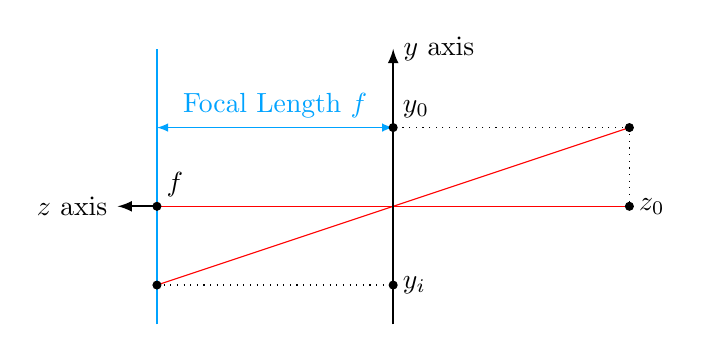
\begin{tikzpicture}
        \draw[red] (3, 0) -- (-3,  0);
        \draw[red] (3, 1) -- (-3, -1);

        \draw[dotted] (3, 1) -- (3, 0) node[right] {$z_0$};
        \draw[dotted] (3, 1) -- (0, 1) node[above right] {$y_0$};
        \draw[dotted] (-3, -1) -- (-3, 0) node[above right] {$f$};
        \draw[dotted] (-3, -1) -- (0, -1) node[right] {$y_i$};

        \draw[thick,-latex] ( 0, -1.5) -- ( 0  , 2) node[right] {$y$ axis};
        \draw[thick,-latex] (-3,  0  ) -- (-3.5, 0) node[left]  {$z$ axis};

        \draw[            lightBlue] (-3, -1.5) -- (-3, 2);
        \draw[latex-latex,lightBlue] (-3,  1  ) -- ( 0, 1) node[midway,above] {Focal Length $f$};

        \filldraw ( 3,  0) circle (0.05);
        \filldraw ( 3,  1) circle (0.05);
        \filldraw ( 0,  1) circle (0.05);
        \filldraw (-3,  0) circle (0.05);
        \filldraw (-3, -1) circle (0.05);
        \filldraw ( 0, -1) circle (0.05);
    \end{tikzpicture}
\end{figure}

From similar triangles, we get \[
    \frac{y_i}{y_0} = \frac{f}{z_0} \implies y_i = \frac{f}{z_0} \cdot y_0
\]

The same applies to 3-dimensional points.

\begin{figure}[ht!]
    \centering
    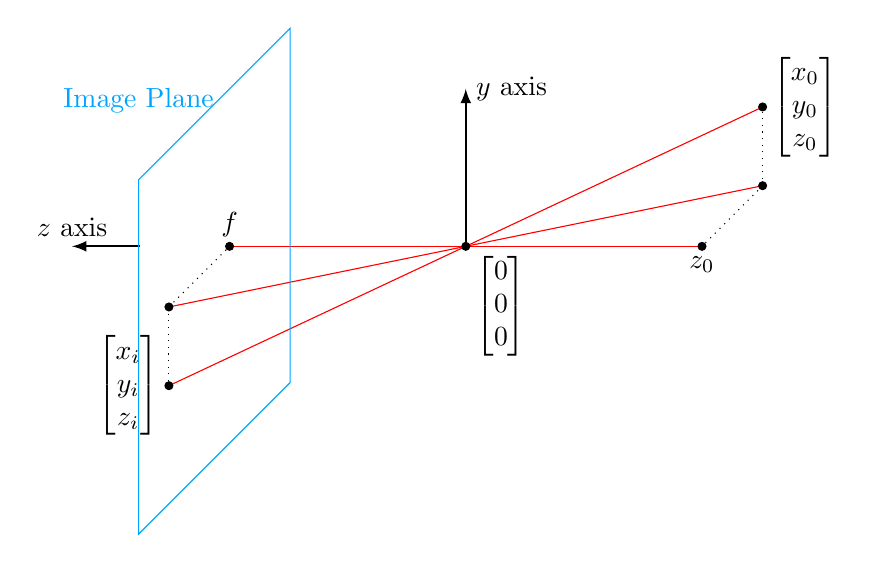
\begin{tikzpicture}
        \draw[red] (3,0, 0) -- (-3, 0,0);
        \draw[red] (3,0,-2) -- (-3, 0,2);
        \draw[red] (3,1,-2) -- (-3,-1,2);

        \draw[dotted] ( 3,0,-2) -- ( 3, 0, 0) node[below] {$z_0$};
        \draw[dotted] ( 3,0,-2) -- ( 3, 1,-2) node[right] {$\begin{bmatrix} x_0 \\ y_0 \\ z_0 \end{bmatrix}$};
        \draw[dotted] (-3,0, 2) -- (-3, 0, 0) node[above] {$f$};
        \draw[dotted] (-3,0, 2) -- (-3,-1, 2) node[left]  {$\begin{bmatrix} x_i \\ y_i \\ z_i \end{bmatrix}$};

        \draw[thick,-latex] ( 0,   0,0) -- ( 0,2,0) node[right] {$y$ axis};
        \draw[thick,-latex] (-4.14,0,0) -- (-5,0,0) node[above] {$z$ axis};

        \draw[lightBlue] (-3,-2.5,-2) -- (-3,2,-2) -- (-3,2,3) -- (-3,-2.5,3) -- cycle;
        \node[lightBlue] at (-3, 3, 3) {Image Plane};

        \filldraw ( 3, 0, 0) circle (0.05);
        \filldraw ( 3, 0,-2) circle (0.05);
        \filldraw ( 3, 1,-2) circle (0.05);
        \filldraw (-3, 0, 0) circle (0.05);
        \filldraw (-3, 0, 2) circle (0.05);
        \filldraw (-3,-1, 2) circle (0.05);

        \node at (0, 0, 0) [below right] {$\begin{bmatrix} 0 \\ 0 \\ 0 \end{bmatrix}$};
        \filldraw (0, 0, 0) circle (0.05);
    \end{tikzpicture}
\end{figure}

We have \[
    \begin{bmatrix} x_i \\ y_i \\ z_i \end{bmatrix} = \frac{f}{z_0} \cdot \begin{bmatrix} x_0 \\ y_0 \\ z_0 \end{bmatrix}
\] Interpretation of homogeneous equality tells us that ``all 3D points have the same projection'', \[
    \begin{bmatrix} x_i \\ y_i \\ z_i \end{bmatrix} \cong \begin{bmatrix} x_0 \\ y_0 \\ z_0 \end{bmatrix}
\] In other words, $\begin{bmatrix} x_i \\ y_i \\ z_i \end{bmatrix}$ represents a ray through the origin. 

\subsubsection{Homogeneous 3D Coordinates}

\begin{figure}[ht!]
    \centering
    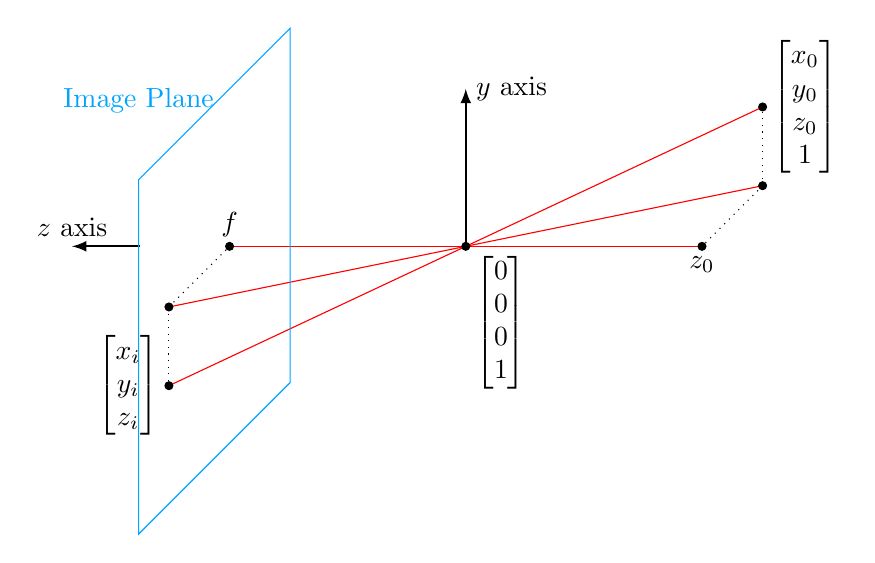
\begin{tikzpicture}
        \draw[red] (3,0, 0) -- (-3, 0,0);
        \draw[red] (3,0,-2) -- (-3, 0,2);
        \draw[red] (3,1,-2) -- (-3,-1,2);

        \draw[dotted] ( 3,0,-2) -- ( 3, 0, 0) node[below] {$z_0$};
        \draw[dotted] ( 3,0,-2) -- ( 3, 1,-2) node[right] {$\begin{bmatrix} x_0 \\ y_0 \\ z_0 \\ 1 \end{bmatrix}$};
        \draw[dotted] (-3,0, 2) -- (-3, 0, 0) node[above] {$f$};
        \draw[dotted] (-3,0, 2) -- (-3,-1, 2) node[left]  {$\begin{bmatrix} x_i \\ y_i \\ z_i \end{bmatrix}$};

        \draw[thick,-latex] ( 0,   0,0) -- ( 0,2,0) node[right] {$y$ axis};
        \draw[thick,-latex] (-4.14,0,0) -- (-5,0,0) node[above] {$z$ axis};

        \draw[lightBlue] (-3,-2.5,-2) -- (-3,2,-2) -- (-3,2,3) -- (-3,-2.5,3) -- cycle;
        \node[lightBlue] at (-3, 3, 3) {Image Plane};

        \filldraw ( 3, 0, 0) circle (0.05);
        \filldraw ( 3, 0,-2) circle (0.05);
        \filldraw ( 3, 1,-2) circle (0.05);
        \filldraw (-3, 0, 0) circle (0.05);
        \filldraw (-3, 0, 2) circle (0.05);
        \filldraw (-3,-1, 2) circle (0.05);

        \node at (0, 0, 0) [below right] {$\begin{bmatrix} 0 \\ 0 \\ 0 \\ 1 \end{bmatrix}$};
        \filldraw (0, 0, 0) circle (0.05);
    \end{tikzpicture}
\end{figure}

Similar to 2D homogeneous coordinates, we can represent 3D points in homogeneous coordinates \[
    \begin{bmatrix} x_0 \\ y_0 \\ z_0 \end{bmatrix} \cong \begin{bmatrix} x_0 \\ y_0 \\ z_0 \\ 1 \end{bmatrix}
\] To convert from the homogeneous coordinates to the Euclidean coordinates, we divide the first three coordinates by the fourth coordinate, i.e. \[
    \begin{bmatrix} x \\ y \\ z \end{bmatrix} = \begin{bmatrix} x_0 \\ y_0 \\ z_0 \end{bmatrix} / w_0
\]

\begin{remark}
    The point \[ \begin{bmatrix} x_0 \\ y_0 \\ z_0 \\ 0 \end{bmatrix} \] is at infinity in 3D space, in the direction of the vector $\begin{bmatrix} x_0 \\ y_0 \\ z_0 \end{bmatrix}$.
\end{remark}

Homogeneous coordinates provide us a convenient way to express the projective of a 3D point into a 2D image, \[
    \begin{bmatrix} x_i \\ y_i \\ 1 \end{bmatrix} = 
    \begin{bmatrix} \frac{f}{z_0} \cdot x_0 \\ \frac{f}{z_0} \cdot y_0 \\ 1 \end{bmatrix} \cong 
    \begin{bmatrix} f & 0 & 0 & 0 \\ 0 & f & 0 & 0 \\ 0 & 0 & 1 & 0 \end{bmatrix} 
    \begin{bmatrix} x_0 \\ y_0 \\ z_0 \\ 1 \end{bmatrix}
\] where $\begin{bmatrix} x_i \\ y_i \\ 1 \end{bmatrix}$ is the homogeneous coordinates of the 2D projection of the 3D point $\begin{bmatrix} x_0 \\ y_0 \\ z_0 \\ 1 \end{bmatrix}$, and the only difference between the 2D and 3D projection matrices is the scaling factor $\frac{f}{z_0}$.

\section{Alignment and Stitching}

% TODO: Add content

\subsection{Estimating Homography from Point Correspondence}

\begin{claim}
    Given sufficiently many point correspondences we can compute tha homogeneous transformation $H$ that aligns two images. We need at least 4 correspondences for a unique solution. 
\end{claim} 

Given a point correspondence $\begin{bmatrix} {x_i}' \\ {y_i}' \\ 1 \end{bmatrix} \cong \begin{bmatrix} x_i \\ y_i \\ 1 \end{bmatrix}$, we can write the following equation \[
    \begin{bmatrix} {x_i}' \\ {y_i}' \\ 1 \end{bmatrix} \cong H \begin{bmatrix} x_i \\ y_i \\ 1 \end{bmatrix}
    \iff
    \begin{bmatrix} {x_i}' \\ {y_i}' \\ 1 \end{bmatrix} \cong \begin{bmatrix} a & b & c \\ d & e & f \\ g & h & 1 \end{bmatrix} \begin{bmatrix} x_i \\ y_i \\ 1 \end{bmatrix}
\] which allows us to establish a system of linear equations \[
    \begin{bmatrix} {x_i}' \\ {y_i}' \\ 1 \end{bmatrix} \cong 
    \begin{bmatrix} ax_i + by_i + c \\ dx_i + ey_i + f \\ gx_i + hy_i + 1 \end{bmatrix} 
    \iff
    \begin{bmatrix} {x_i}' \\ {y_i}' \\ 1 \end{bmatrix} \cong 
    \begin{bmatrix} {ax_i + by_i + c}/{gx_i + hy_i + 1} \\ {dx_i + ey_i + f}/{gx_i + hy_i + 1} \\ 1 \end{bmatrix} 
\]

That is, one correspondence gives us two linear equations. We have 8 unknowns, so we need 4 correspondences to solve the system of linear equations.

\section{3D Metrology}

\subsection{3D Reconstruction from 2D Images}

% TODO: Football example

\subsection{Vanishing Points}

\begin{definition}
    A \term{vanishing point} is a point on the image plane of a perspective rendering where the two-dimensional perspective projections of mutually parallel lines in three-dimensional space appear to converge. 
\end{definition}

\begin{figure}[ht!]
    \centering

    \begin{subfigure}{0.45\linewidth}
        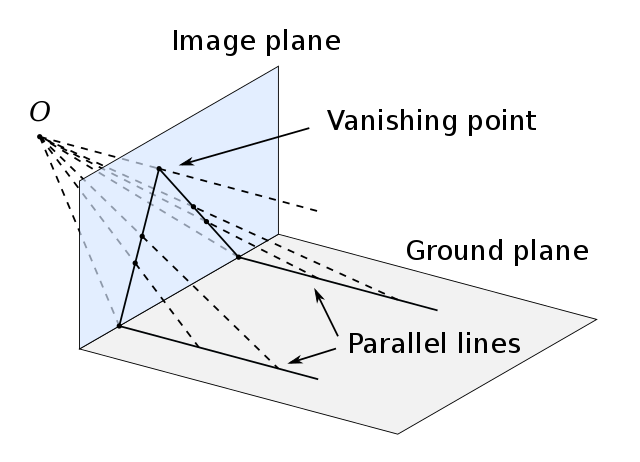
\includegraphics[width=\linewidth]{figures/640px-Vanishing_point.svg.png}
        % TODO: cite https://pxhere.com/en/photo/734310
    \end{subfigure}
    \hfil%
    \begin{subfigure}{0.45\linewidth}
        
\includegraphics[width=\linewidth]{figures/nature-forest-track-railway-railroad-bridge-734310-pxhere.com.jpg}
        % TODO: cite https://commons.wikimedia.org/wiki/File:Vanishing_point.svg
    \end{subfigure}

\end{figure}

Every direction in space has a unique vanishing point. These vanishing points are the intersection of the image plane with the projective space, and they all lie on the horizon line.

\chapter{Image Filtering}

\section{Linear Shift-Invariant Filters}

\subsection{Definition}

A filter transforms one signal into another. Filters are used to describe image formation (lens burring, sensor noise, etc.), as well as to implement operations on images (edge detection, noise reduction, etc.).

\begin{figure}[ht!]
    \centering
    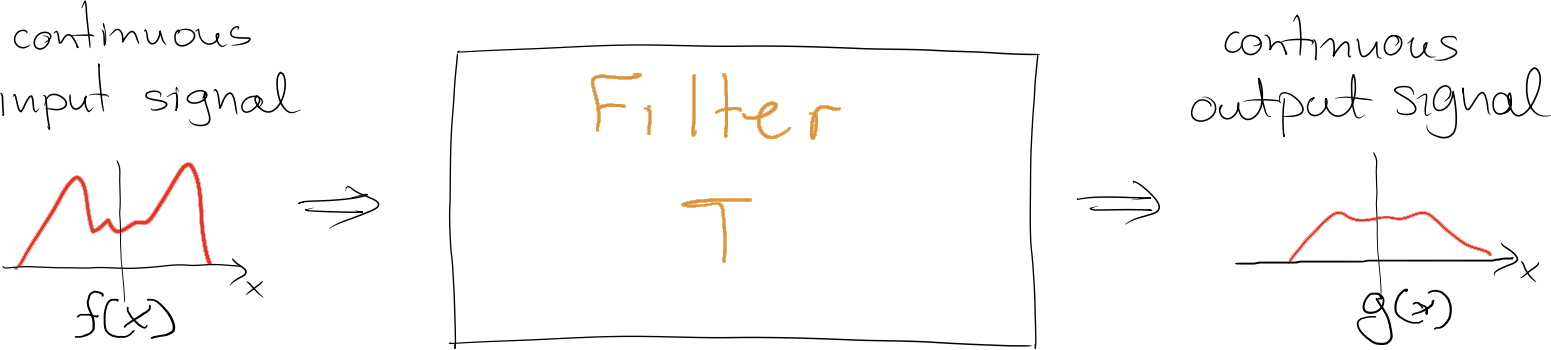
\includegraphics[width=0.75\linewidth]{figures/filter.png}
\end{figure}

\begin{definition}[Linear Transformation]\index{Linear Transformation}\label{def:linear-transformation}
    A transformation $T$ is \term{linear} if and only if it satisfies \[
        T[a_1 f_1(x) + a_2 f_2(x)] = a_1 T[f_1(x)] + a_2 T[f_2(x)]
    \] for any $a_1, a_2 \in \mathbb{R}$ and continuous functions $f_1, f_2$. 
\end{definition}

Every linear transformation between functions $f, g$ can be expressed as an integral of the form \[
    g(x) = \int_{-\infty}^{\infty} h(x, \tau) f(\tau) \, d\tau,
\] where the $h(x, \tau)$ is the contribution of position $\tau$ of the input to position $x$ of the output.

% TODO: Add a figure to illustrate shift-invariance

\begin{definition}[Shift-Invariant Filter]\index{Shift-Invariant Filter}\label{def:shift-invariant-filter}
    A filter $h(x, \tau)$ is \term{shift-invariant} if and only if shifted inputs produce identical but shifted outputs. 
\end{definition}

% TODO: Graph of the two functions

Imagine we have the shifted input \[
    f'(x') = f(x - x_0)
\] and the shifted output \[
    g'(x') = g(x - x_0).
\] The \term{shift invariance property} states that \[
    T[f(x - x_0)] = g(x - x_0)
\]

\subsection{The Impulse Function}

\chapter{Model Fitting}

\chapter{Color Imaging and Displaying}

\part{Image Representation for CV}

\chapter{Continuous}

\chapter{Vector-Based}

\chapter{Multi-Scale}

\part{Appendices}

\chapter*{Bibliography}
\addcontentsline{toc}{part}{Bibliography}
\nocite{*}
\printbibliography[heading=bibempty]

\cleardoublepage
\phantomsection
\setlength{\columnsep}{0.75cm}
\addcontentsline{toc}{part}{Index}
\printindex

\end{document}